\begin{figure}[htb]
\centering
\small

\ifTIKZFIG
\begin{tikzpicture}\small

% =========================================================
% 時間軸
% =========================================================
\ifJPN
\draw[thick,->,>=stealth,line width=.3mm]
  (0,0) -- (14,0)
  node[anchor=north] {時間（Time）};
\else
\draw[thick,->,>=stealth,line width=.3mm]
  (0,0) -- (14,0)
  node[anchor=north] {Time};
\fi

% =========================================================
% 適用範囲
% =========================================================

% Immediate Grammar
\draw[thick,draw=red]
  (2.05,.08) -- (6.95,.08);

% Adjustive Grammar
% IG終了以前に開始する
\draw[thick,draw=blue]
  (5.55,-.08) -- (11.95,-.08);

% =========================================================
% 非言語状態
% =========================================================
\ifJPN
\node[anchor=south] at (1,1.0)
  {\parbox{25mm}{\centering 非言語状態}};
\else
\node[anchor=south] at (1,1.4)
  {\parbox{30mm}{\centering Non-language\\state}};
\fi

% =========================================================
% Pre-boundary
% =========================================================
\ifJPN
\node[anchor=south] at (2,1.0)
  {\parbox{35mm}{\centering
    前限界\\
    Pre-boundary\\
    （言語処理開始）}};
\else
\node[anchor=south] at (2,1.4)
  {\parbox{38mm}{\centering
    Pre-boundary\\
    Language processing begins}};
\fi

% =========================================================
% AG Pre-boundary
% =========================================================
\ifJPN
\node[anchor=south] at (5.5,1.0)
  {\parbox{40mm}{\centering
    調整文法の前限界\\
    AG Pre-boundary\\
    （調整の介入開始）}};
\else
\node[anchor=south] at (5.5,1.4)
  {\parbox{43mm}{\centering
    AG Pre-boundary\\
    Adjustive intervention begins}};
\fi

% =========================================================
% IG Post-boundary
% =========================================================
\ifJPN
\node[anchor=south] at (7,1.0)
  {\parbox{38mm}{\centering
    即時文法の後限界\\
    IG Post-boundary}};
\else
\node[anchor=south] at (7,1.4)
  {\parbox{38mm}{\centering
    IG Post-boundary}};
\fi

% =========================================================
% AG Post-boundary / Saturation Point
% =========================================================
\ifJPN
\node[anchor=south] at (12,1.0)
  {\parbox{45mm}{\centering
    調整文法の後限界\\
    ＝調整飽和点\\
    Saturation Point}};
\else
\node[anchor=south] at (12,1.4)
  {\parbox{50mm}{\centering
    AG Post-boundary\\
    = Adjustive Saturation Point}};
\fi

% =========================================================
% 範囲ラベル
% =========================================================
\ifJPN
\node at (3.75,.55)
  {\parbox{34mm}{\centering
    即時文法の適用範囲\\
    Immediate Grammar}};
\else
\node at (3.75,.55)
  {\parbox{38mm}{\centering
    Application Range of\\
    Immediate Grammar}};
\fi

\ifJPN
\node at (9.5,-.55)
  {\parbox{34mm}{\centering
    調整文法の適用範囲\\
    Adjustive Grammar}};
\else
\node at (9.5,-.55)
  {\parbox{38mm}{\centering
    Application Range of\\
    Adjustive Grammar}};
\fi

% =========================================================
% Overlap
% =========================================================
\ifJPN
\node at (6.25,-.55)
  {\parbox{28mm}{\centering
    重複区間\\
    Overlap}};
\else
\node at (6.25,-.55)
  {\parbox{28mm}{\centering
    Overlap}};
\fi

% =========================================================
% 境界を示す縦破線
% =========================================================
\ifJPN
\draw[dashed,<-,>=stealth,line width=.3mm]
  (2,.16) -- (2,1.0);

\draw[dashed,<-,>=stealth,line width=.3mm]
  (5.5,.16) -- (5.5,1.0);

\draw[dashed,<-,>=stealth,line width=.3mm]
  (7,.16) -- (7,1.0);

\draw[dashed,<-,>=stealth,line width=.3mm]
  (12,.03) -- (12,1.0);
\else
\draw[dashed,<-,>=stealth,line width=.3mm]
  (2,.16) -- (2,1.4);

\draw[dashed,<-,>=stealth,line width=.3mm]
  (5.5,.16) -- (5.5,1.4);

\draw[dashed,<-,>=stealth,line width=.3mm]
  (7,.16) -- (7,1.4);

\draw[dashed,<-,>=stealth,line width=.3mm]
  (12,.03) -- (12,1.4);
\fi

% =========================================================
% 時間軸上のマーカー
% =========================================================

% Pre-boundary: language processing begins
\fill (2,.08) circle (2pt);

% AG Pre-boundary
\fill (5.5,-.08) circle (2pt);

% IG Post-boundary
\draw[fill=white] (7,.08) circle (2pt);

% AG Post-boundary / Saturation
\fill (12,-.08) circle (2pt);

\end{tikzpicture}

\else

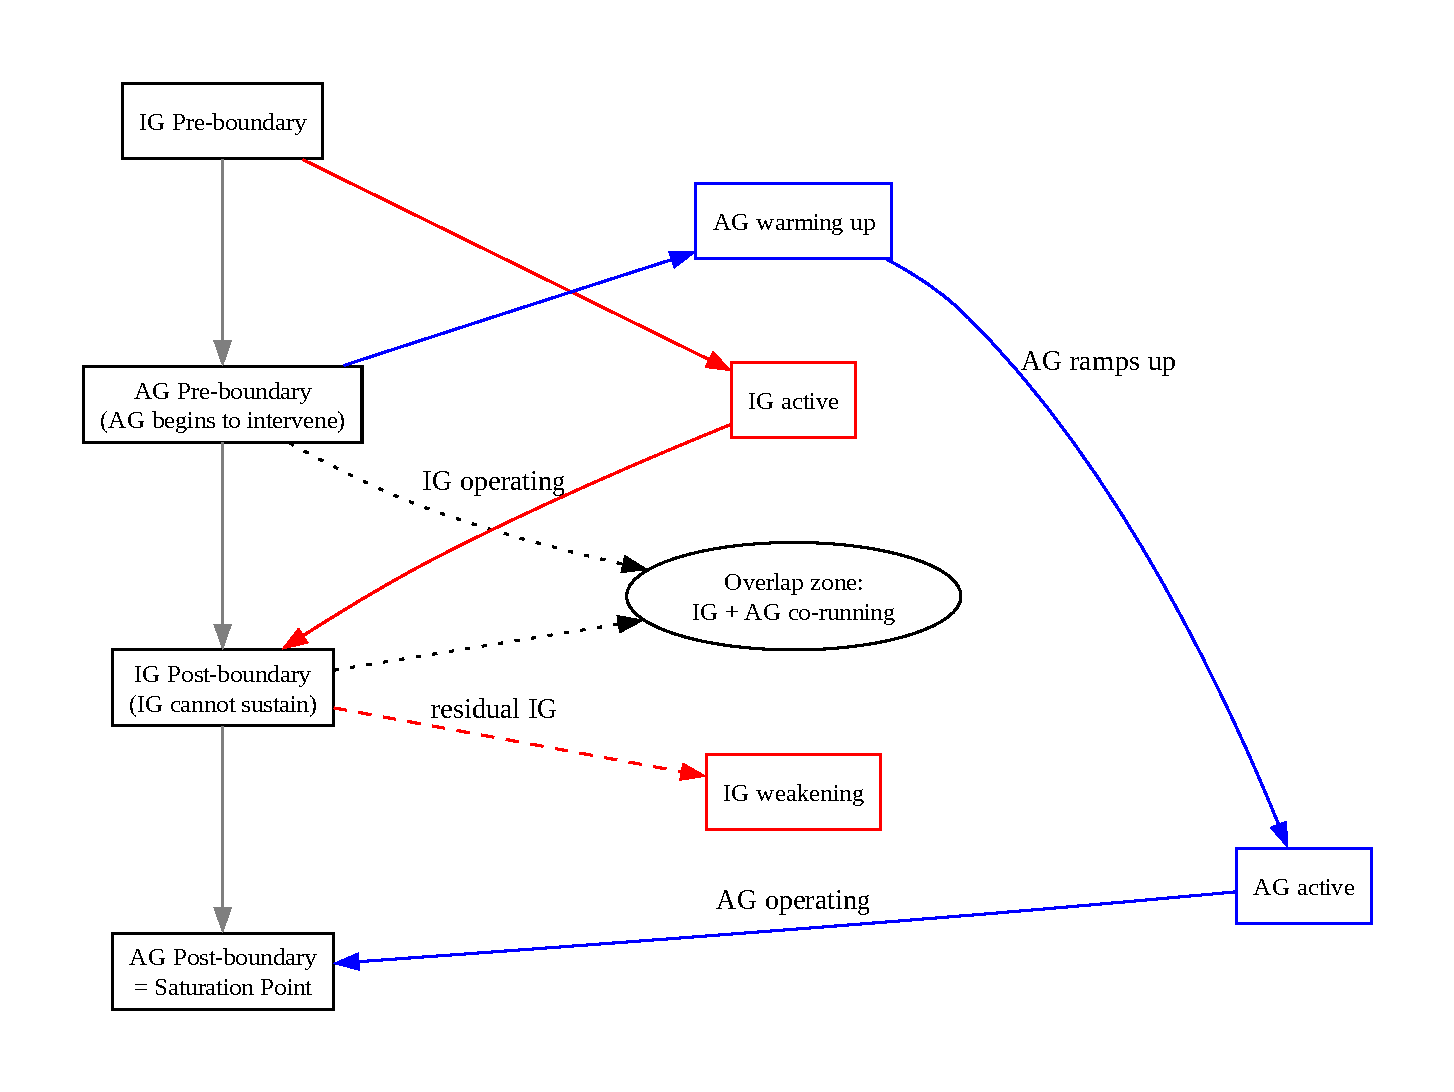
\includegraphics[width=0.95\textwidth]{pgm-fig-concept.pdf}

\fi

\ifJPN
\caption{即時文法と調整文法の限界と重複区間}
\label{fig:boundary-j}
\else
\caption{Boundaries and overlap between Immediate Grammar and Adjustive Grammar}
\label{fig:boundary}
\fi

\end{figure}
